% TUL — Thought Unpack Loop (mechanism). Spec: docs/tul-spec.md.
% Star of the show: loop once per thought (slot), freeze z, AR-decode the next
% span with z kept in the shared sequence. Exit is the punct / cap rule — no
% learned exit gate in v1 (spec §3.5 / §6).
% Palette follows morph_overview.tex (Paul Tol).
% Compile: pdflatex tul_mechanism.tex
%          pdftoppm -png -r 220 -singlefile tul_mechanism.pdf ../tul_mechanism
% Supersedes: tul_overview.tex (deprecated).

\documentclass[border=14pt]{standalone}
\usepackage[T1]{fontenc}
\usepackage{amsmath,amssymb}
\usepackage{tikz}
\usetikzlibrary{arrows.meta, fit, positioning, calc, backgrounds,
  decorations.pathreplacing, bending}

\definecolor{cbBlue}{HTML}{4477AA}
\definecolor{cbOrange}{HTML}{EE7733}
\definecolor{cbPurple}{HTML}{AA3377}
\definecolor{cbTeal}{HTML}{228833}
\definecolor{fBlue}{HTML}{DCEAF7}
\definecolor{fOrange}{HTML}{FDE8D0}
\definecolor{fPurple}{HTML}{EEDCEE}
\definecolor{fTeal}{HTML}{D4EDDA}
\definecolor{fGray}{HTML}{EBEBEB}
\definecolor{bdr}{HTML}{555555}
\definecolor{loopC}{HTML}{2255AA}

\tikzset{
  B/.style={draw=bdr, thick, rounded corners=4pt, minimum width=11.2cm,
    minimum height=1.05cm, font=\small\sffamily, align=center, inner sep=7pt},
  tok/.style={draw=bdr, fill=fGray, minimum width=0.78cm, minimum height=0.68cm,
    font=\footnotesize\sffamily, inner sep=1pt},
  tokDone/.style={draw=cbTeal, thick, fill=fTeal, minimum width=0.78cm,
    minimum height=0.68cm, font=\footnotesize\sffamily\bfseries, inner sep=1pt,
    text=cbTeal!70!black},
  tokNext/.style={draw=cbOrange!70!black, thick, fill=fOrange!55, minimum width=0.78cm,
    minimum height=0.68cm, font=\footnotesize\sffamily, inner sep=1pt,
    text=cbOrange!75!black},
  punct/.style={draw=cbOrange, very thick, fill=fOrange, minimum width=0.78cm,
    minimum height=0.68cm, font=\footnotesize\sffamily\bfseries, inner sep=1pt,
    text=cbOrange!75!black},
  slot/.style={draw=cbPurple, thick, fill=fPurple, minimum width=0.78cm,
    minimum height=0.68cm, font=\footnotesize\sffamily\bfseries, inner sep=1pt},
  A/.style={-{Stealth[length=2.5mm,width=2mm]}, thick},
  sub/.style={font=\scriptsize\sffamily},
  src/.style={font=\scriptsize\sffamily, text=bdr, align=center},
  ph/.style={font=\small\sffamily\bfseries},
}

\begin{document}
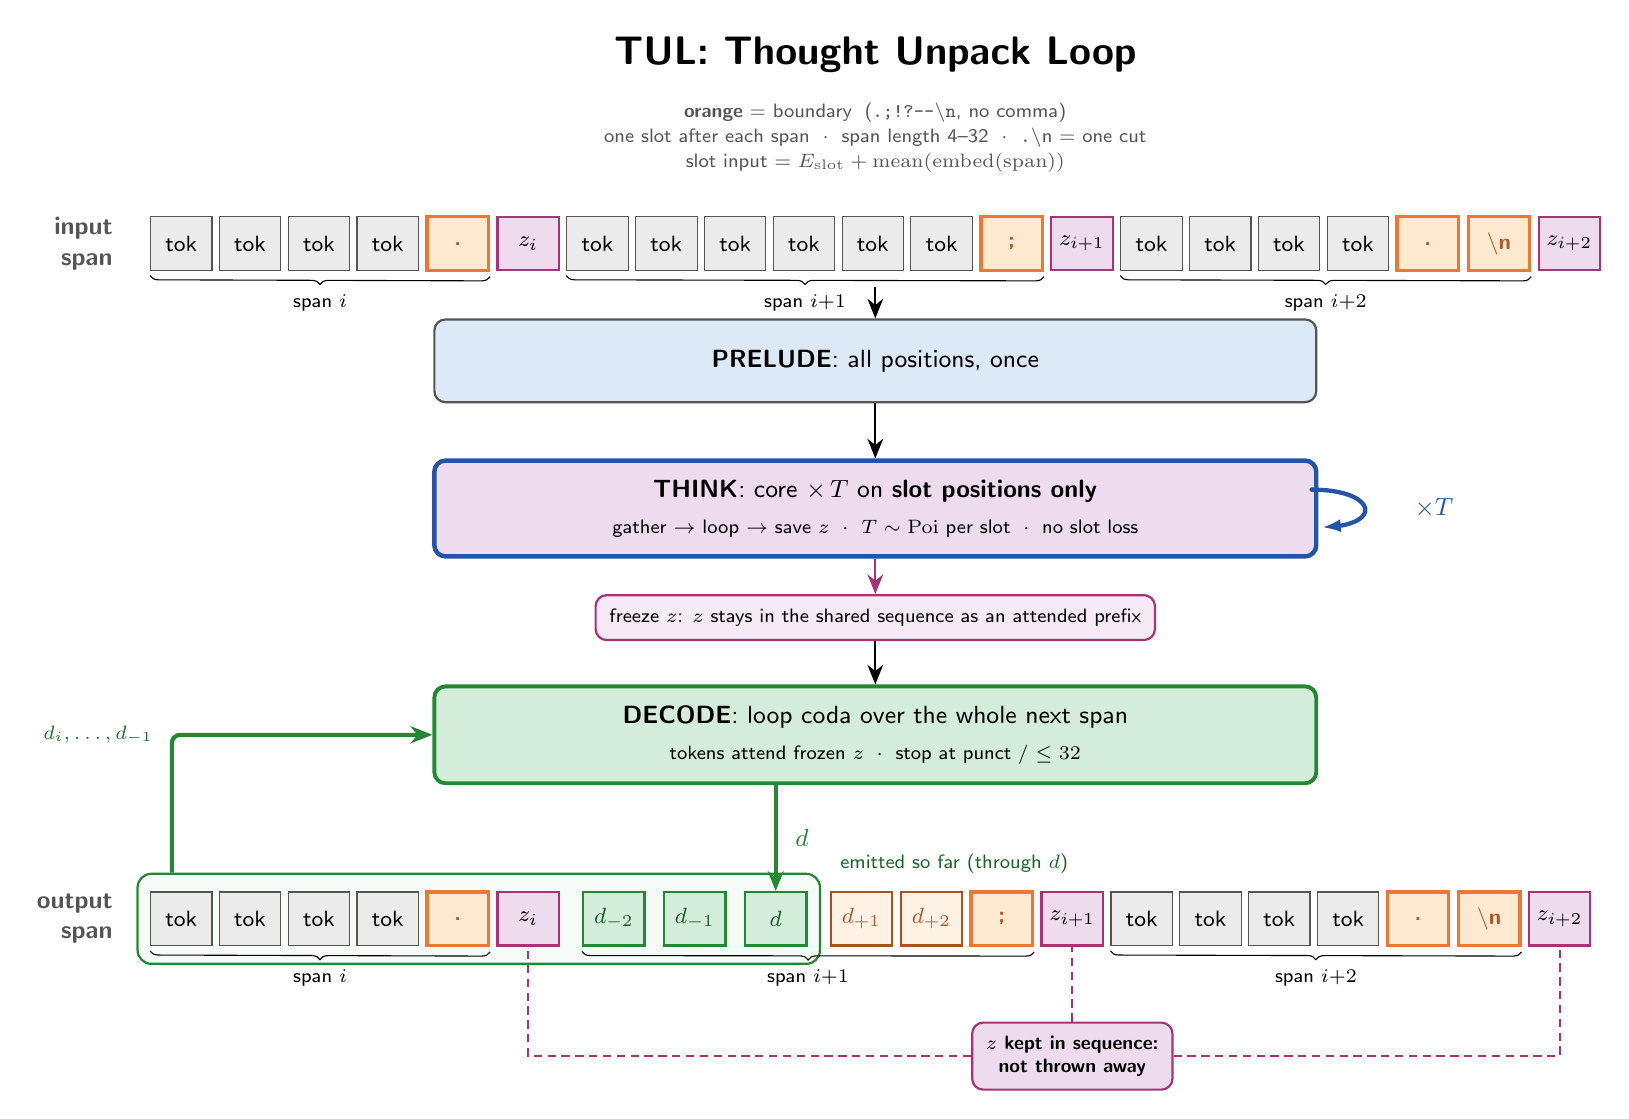
\begin{tikzpicture}[node distance=0.55cm]

% ── INPUT SEQUENCE (built first so the title can center on it) ──────────────
\node[tok] (a1) {tok};
\node[tok, right=0.08cm of a1] (a2) {tok};
\node[tok, right=0.08cm of a2] (a3) {tok};
\node[tok, right=0.08cm of a3] (a4) {tok};
\node[punct, right=0.08cm of a4] (a5) {.};
\node[slot, right=0.08cm of a5] (az1) {$z_i$};
\node[tok, right=0.08cm of az1] (a6) {tok};
\node[tok, right=0.08cm of a6] (a7) {tok};
\node[tok, right=0.08cm of a7] (a8) {tok};
\node[tok, right=0.08cm of a8] (a9) {tok};
\node[tok, right=0.08cm of a9] (a10) {tok};
\node[tok, right=0.08cm of a10] (a10b) {tok};
\node[punct, right=0.08cm of a10b] (a11) {;};
\node[slot, right=0.08cm of a11] (az2) {$z_{i+1}$};
\node[tok, right=0.08cm of az2] (a12) {tok};
\node[tok, right=0.08cm of a12] (a13) {tok};
\node[tok, right=0.08cm of a13] (a14) {tok};
\node[tok, right=0.08cm of a14] (a14b) {tok};
\node[punct, right=0.08cm of a14b] (a15) {.};
\node[punct, right=0.08cm of a15] (a16) {\textbackslash n};
\node[slot, right=0.08cm of a16] (az3) {$z_{i+2}$};

\node[ph, text=bdr, left=0.35cm of a1, align=right] {input\\span};

% horizontal center of the in-row (notation sits on this)
\coordinate (amid) at ($(a1.center)!0.5!(az3.center)$);

% notation ABOVE the span (centered on the in-row)
\node[src] (rule) at ($(amid)+(0,1.35)$) {%
  \textbf{orange} = boundary \;(\texttt{.;!?--\textbackslash n}, no comma)\\[1pt]
  one slot after each span \;$\cdot$\; span length 4--32 \;$\cdot$\; \texttt{.}\textbackslash n = one cut\\[1pt]
  slot input $= E_{\mathrm{slot}} + \mathrm{mean}(\mathrm{embed}(\mathrm{span}))$};

% title centered with the main column (span / notation / blocks)
\node[font=\Large\sffamily\bfseries] (title) at ($(amid)+(0,2.40)$)
  {TUL: Thought Unpack Loop};

\draw[decorate, decoration={brace, mirror, amplitude=3pt}]
  ($(a1.south west)+(0,-0.06)$) -- ($(a5.south east)+(0,-0.06)$)
  node[midway, below=3pt, sub] {span $i$};
\draw[decorate, decoration={brace, mirror, amplitude=3pt}]
  ($(a6.south west)+(0,-0.06)$) -- ($(a11.south east)+(0,-0.06)$)
  node[midway, below=3pt, sub] {span $i{+}1$};
\draw[decorate, decoration={brace, mirror, amplitude=3pt}]
  ($(a12.south west)+(0,-0.06)$) -- ($(a16.south east)+(0,-0.06)$)
  node[midway, below=3pt, sub] {span $i{+}2$};

% ── PRELUDE (centered on the span midpoint, not on a9) ──────────────────────
\node[B, fill=fBlue, below=0.95cm of amid] (pre) {%
  \textbf{PRELUDE}: all positions, once};
% arrow starts below span braces so it does not cut the brace labels
\draw[A] ($(amid)-(0,0.55)$) -- (pre.north);

% ── THINK ───────────────────────────────────────────────────────────────────
\node[B, fill=fPurple, draw=loopC, line width=1.6pt, below=0.7cm of pre] (think) {%
  \textbf{THINK}: core $\times\,T$ on \textbf{slot positions only}\\[2pt]
  {\scriptsize gather $\to$ loop $\to$ save $z$ \;$\cdot$\; $T\sim\mathrm{Poi}$ per slot \;$\cdot$\; no slot loss}};
\draw[A] (pre.south) -- (think.north);

% ×T loop: out=0/in=0 U-turn; start tucked under the border; flex'+shorten
% on the tip (the old orthogonal Stealth path left a shaft nub).
\draw[loopC, line width=1.55pt, line cap=round, shorten >=1.2pt,
      -{Latex[length=2.4mm, width=1.65mm, flex']}]
  ([xshift=-2.5pt, yshift=2.4mm]think.east)
    to[out=0, in=0, min distance=8.5mm]
  ([yshift=-2.4mm]think.east);
\node[font=\small\sffamily\bfseries, text=loopC, anchor=west]
  at ([xshift=11mm]think.east) {$\times T$};

% freeze annotation
\node[draw=cbPurple, thick, rounded corners=4pt, fill=fPurple!60,
      font=\scriptsize\sffamily, inner sep=5pt, align=center,
      below=0.45cm of think] (freeze) {%
  freeze $z$: $z$ stays in the shared sequence as an attended prefix};
\draw[A, draw=cbPurple] (think.south) -- (freeze.north);

% ── DECODE ↔ span (AR feedback; distinct from THINK ×T) ─────────────────────
\node[B, fill=fTeal, draw=cbTeal, line width=1.4pt, below=0.55cm of freeze] (dec) {%
  \textbf{DECODE}: loop coda over the whole next span\\[2pt]
  {\scriptsize tokens attend frozen $z$ \;$\cdot$\; stop at punct / $\le 32$}};
\draw[A] (freeze.south) -- (dec.north);

% ── OUTPUT SEQUENCE (bottom) — same x as the in-row ─────────────────────────
\coordinate (bout) at (a1 |- dec.south);
\node[tok, below=1.35cm of bout] (b1) {tok};
\node[tok, right=0.08cm of b1] (b2) {tok};
\node[tok, right=0.08cm of b2] (b3) {tok};
\node[tok, right=0.08cm of b3] (b4) {tok};
\node[punct, right=0.08cm of b4] (b5) {.};
\node[slot, right=0.08cm of b5] (bz1) {$z_i$};
% active span: emitted so far (z_i plan + toks through current d); future stays outside the box
\node[tokDone, right=0.28cm of bz1] (b6) {$d_{-2}$};
\node[tokDone, right=0.22cm of b6] (b7) {$d_{-1}$};
\node[tokDone, right=0.22cm of b7] (b8) {$d$};
\node[tokNext, right=0.28cm of b8] (b9) {$d_{+1}$};
\node[tokNext, right=0.08cm of b9] (b10) {$d_{+2}$};
\node[punct, right=0.08cm of b10] (b11) {;};
\node[slot, right=0.08cm of b11] (bz2) {$z_{i+1}$};
\node[tok, right=0.08cm of bz2] (b12) {tok};
\node[tok, right=0.08cm of b12] (b13) {tok};
\node[tok, right=0.08cm of b13] (b14) {tok};
\node[tok, right=0.08cm of b14] (b14b) {tok};
\node[punct, right=0.08cm of b14b] (b15) {.};
\node[punct, right=0.08cm of b15] (b16) {\textbackslash n};
\node[slot, right=0.08cm of b16] (bz3) {$z_{i+2}$};

\node[ph, text=bdr, left=0.35cm of b1, align=right] {output\\span};

% frame = everything emitted so far (span toks + punct + z_i + … + current d)
\begin{scope}[on background layer]
  \node[draw=cbTeal, thick, rounded corners=5pt, fill=fTeal!20,
        fit=(b1)(b2)(b3)(b4)(b5)(bz1)(b6)(b7)(b8),
        inner xsep=4.5pt, inner ysep=6pt] (spanBox) {};
\end{scope}
\node[sub, text=cbTeal!75!black, anchor=west]
  at ($(spanBox.north east)+(0.12,0.12)$) {emitted so far (through $d$)};

% d: vertical drop from DECODE's bottom edge aligned over $d$ (no diagonal)
\draw[A, draw=cbTeal, line width=1.5pt]
  (dec.south -| b8) -- (b8.north)
  node[midway, right=3pt, font=\small\sffamily\bfseries, text=cbTeal] {$d$};

% feedback: leave from the TOP edge (near left), straight up, then into DECODE
\coordinate (fbStart) at ([xshift=0.45cm]spanBox.north west);
\draw[cbTeal, line width=1.5pt, rounded corners=3pt,
      -{Stealth[length=2.8mm,width=2.2mm]}]
  (fbStart) |- (dec.west);
\node[font=\scriptsize\sffamily, text=cbTeal!80!black, anchor=east]
  at ([xshift=-0.12cm]fbStart |- dec.west) {$d_{i},\ldots,d_{-1}$};

% braces: span i+1 is the full token run including future + punct
\draw[decorate, decoration={brace, mirror, amplitude=3pt}]
  ($(b1.south west)+(0,-0.06)$) -- ($(b5.south east)+(0,-0.06)$)
  node[midway, below=3pt, sub] {span $i$};
\draw[decorate, decoration={brace, mirror, amplitude=3pt}]
  ($(b6.south west)+(0,-0.06)$) -- ($(b11.south east)+(0,-0.06)$)
  node[midway, below=3pt, sub] {span $i{+}1$};
\draw[decorate, decoration={brace, mirror, amplitude=3pt}]
  ($(b12.south west)+(0,-0.06)$) -- ($(b16.south east)+(0,-0.06)$)
  node[midway, below=3pt, sub] {span $i{+}2$};

% Sit UNDER z_{i+1} so z_i is left of west and z_{i+2} is right of east.
% TikZ: (A -| B) = (B.x, A.y); (A |- B) = (A.x, B.y). Side L-exits need -|.
\node[draw=cbPurple, thick, rounded corners=4pt, fill=fPurple,
      font=\scriptsize\sffamily\bfseries, align=center, inner sep=5pt,
      below=0.95cm of bz2] (kept)
  {$z$ kept in sequence:\\not thrown away};
% left → z_i: leave WEST mid, go left, then up (one bend)
\draw[cbPurple, thick, densely dashed]
  (kept.west) -| (bz1.south);
% middle → z_{i+1}: straight up from TOP of kept (box sits under this slot)
\draw[cbPurple, thick, densely dashed]
  (kept.north) -- (bz2.south);
% right → z_{i+2}: leave EAST mid, go right, then up (one bend)
\draw[cbPurple, thick, densely dashed]
  (kept.east) -| (bz3.south);

\end{tikzpicture}
\end{document}
